%%%%%%%%%%%%%%%%%%%%%%%%%%%%%%%%%%%%%%%%%%%%%%%%%%%%%%%%%%%%%%%%%%%%%%%%%%%%%%%%%%%%%%%%%%%%%%%
%Plantilla: para la realizaci�n de informes.
%Curso:     Simulaci�n estad�stica.
%Profesor:  Johann A. Ospina.
%%%%%%%%%%%%%%%%%%%%%%%%%%%%%%%%%%%%%%%%%%%%%%%%%%%%%%%%%%%%%%%%%%%%%%%%%%%%%%%%%%%%%%%%%%%%%%%


%Establece el tipo de documento (art�culo), tama�o de letra (10pt) a una columna.
\documentclass[letterpaper,12pt,onecolumn,titlepage]{article} 
 
 
% Cargar paquetes
\usepackage{verbatim}
\usepackage{mathrsfs}
\usepackage{amsmath}
\usepackage{amssymb}
\usepackage{subfigure}
\usepackage{ucs}
\usepackage[latin1]{inputenc}
\usepackage[spanish]{babel}
\usepackage{fontenc}
\usepackage{graphicx}
\usepackage{anysize}
\usepackage{fancyhdr}
\usepackage[comma,authoryear]{natbib}
\usepackage{url} %paquete para definir url
\usepackage{hyperref}  %hipervinculos

%Estilo de la p�gina
\pagestyle{fancy}

%Establecer el margen
\marginsize{2cm}{2cm}{1cm}{1cm}
\setlength{\headheight}{13.1pt}


% Portada
\title{
    \textbf{Laboratorio N.3}\
    ~\\{Introduccion a Los Metodos Estadisticos}   
    ~\\{Estimacion por intervalos y simulacion}}
\author{
    {Diana Carolina Arias Sinisterra Cod. 1528008}
 ~\\{Kevin Steven Garcia Chica Cod. 1533173}
 ~\\{Cesar Andres Saavedra Vanegas Cod. 1628466}}

\date{
     \textbf{Universidad Del Valle}\   
    ~\\{Facultad De Ingenieria}
    ~\\{Estadistica}
    ~\\{Octubre}
    ~\\{2017}}
 
 
 
\decimalpoint %Poner punto decimal
 
\begin{document}
 
% Se aplica el formato a las p�ginas. Se despliegan: portada e �ndices de materias, figuras y tablas
\renewcommand{\listtablename}{}
\renewcommand{\tablename}{Tabla}
\maketitle
\setcounter{page}{2}
\tableofcontents{}
%\thispagestyle{empty}
%\newpage
%\listoffigures{}
%\listoftables

\thispagestyle{empty}

\newpage
\fancyhead{}
\fancyfoot{}
 
% Encabezado y pie de pagina
\lhead{Introduccion a los Metodos Estadisticos}
\lfoot{Universidad Del Valle}
\rfoot{\thepage}

% Estilo de la bibliograf�a
\bibliographystyle{apalike}
 
% Desarrollo de los contenidos del documento
\pagebreak\section{Situaci\'{o}n 1}
\subsection{Punto a.}

~\\ \begin{center}
 \begin{tabular}{|c|c|c|c|c|c|c|c|c|c|c|c|c|}
\hline 
\rule[-1ex]{0pt}{2.5ex} ANTES & 12 & 10 & 15 & 8 & 19 & 14 & 12 & 21 & 16 & 11 & 8 & 15 \\ 
\hline 
\rule[-1ex]{0pt}{2.5ex} DESPUES & 11 & 11 & 17 & 9 & 21 & 13 & 16 & 25 & 20 & 18 & 10 & 17 \\ 
\hline 
\rule[-1ex]{0pt}{2.5ex} DIFERENCIA & 1 & -1 & -2 & -1 & -2 & 1 & -4 & -4 & -4 & -7 & -2 & -2 \\ 
\hline 
\end{tabular} 
\end{center}

\subsection{Punto b.}


\pagebreak\section{Situaci\'{o}n 2}
~\\ Para darnos cuenta que en realidad la mayoria de personas aprueba el proyecto de fluoracion del agua, debemos encontrar un intervalo de confianza de la proporcion de personas que estan a favor, y ver si este esta por encima del 0.5.
~\\ Entonces. Tomando los datos del enunciado tenemos:
~\\ $n=200$, $\hat{P}=\frac{110}{200}=0.55$ (Proporcicion de personas a favor), $\alpha=0.01$ entonces $1-\alpha=0.99$
~\\ Ahora, para encontrar un intervalo de confianza para la proporcion, aplicamos la siguiente formula:

~\\ $IC(P)_{(1-\alpha)\%}=\left[\hat{P}-Z_{1-\frac{\alpha}{2}}\sqrt{\frac{\hat{P}(1-\hat{P}}{n}};\hat{P}+Z_{1-\frac{\alpha}{2}}\sqrt{\frac{\hat{P}(1-\hat{P}}{n}}\right]$

~\\ Reemplazando en la formula, tenemos:

~\\ $IC(P)_{99\%}=\left[0.55-Z_{0.995}\sqrt{\frac{0.55(0.45)}{200}};0.55+Z_{0.995}\sqrt{\frac{0.55(0.45)}{200}}\right]$

~\\ $IC(P)_{99\%}=[0.55-2.5758(0.035178) ; 0.55+2.5758(0.035178)]$

~\\ $IC(P)_{99\%}=[0.4594 ; 0.6406]$

~\\ \textbf{INTERPRETACION:}
 \begin{figure}[!h]
    \begin{center}
        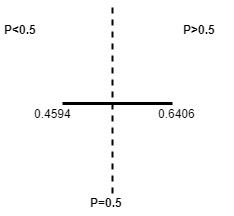
\includegraphics[width=10cm]{Figuras/Grafico1.png}
        \caption{Interpretacion intervalo para proporciones}
        \label{fig:Densidad}
    \end{center}
\end{figure}

~\\ Como asignamos una confianza del $99\%$ a nuestro intervalo, decimos que el $99\%$ de las veces que se repita el experimento, la proporcion real de personas que estan a favor de que se agregue fluoruro de sodio al agua va a caer en dicho intervalo (entre 0.4594 y 0.6406). Ahora, observando la grafica, podemos ver que en el intervalo esta contenida la probabilidad de 0.5, por lo tanto, la muestra no nos da evidencia para decir que la mayoria de personas aprueba el proyecto de fluoracion.

\pagebreak\section{Situaci\'{o}n 3}
\subsection{Punto a.}
 \begin{figure}[!h]
    \begin{center}
        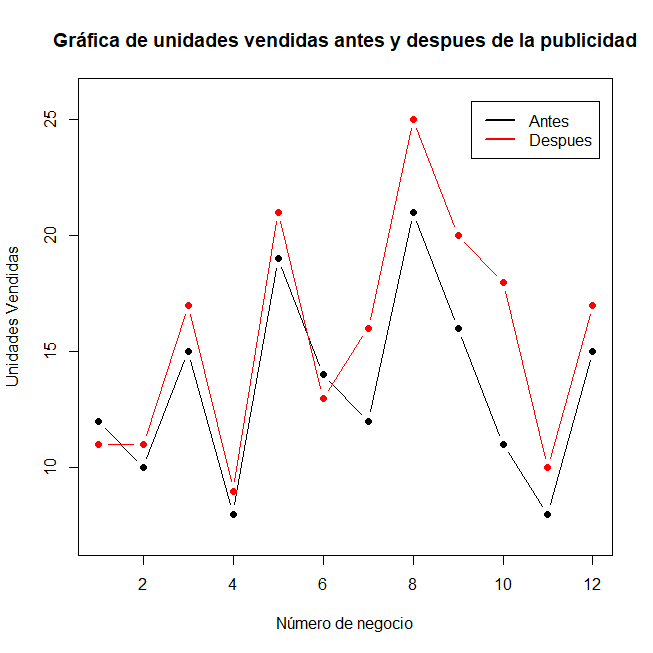
\includegraphics[width=10cm]{Figuras/Grafico2.png}
        \caption{Grafico de puntos y lineas por negocio de unidades vendidas, antes y despues de la publicidad}
        \label{fig:Densidad}
    \end{center}
\end{figure}

~\\ En el analisis exploratorio de datos que se elaboro, encontramos que la mejor grafica para mostrar la efectividad de la campana publicitaria fue la grafica de puntos y lineas. El eje x son cada una de las sucursales o negocios, y el eje y son las unidades vendidas. La linea negra representa las unidades que se vendian en dichos negocios antes de la campana publicitaria, y la roja representa las unidades vendidas despues de la campana.
~\\ Podemos observar que en solo dos de los negocios la linea negra esta por encima de la blanca, es decir, se vendieron mas articulos antes de la campana que despues de ella; en el resto de negocios (10 negocios)la linea roja esta por encima de la negra, es decir,se vendieron mas articulos despues de la campana que antes de ella. Ademas, si miramos detalladamente las diferencias en los negocios en los cuales la linea negra esta por encima de la roja son de tan solo una unidad vendida, en cambio en los negocios en los cuales la linea roja esta por encima de la negra, hay diferencia hasta de 7 unidades vendidas.
~\\ \textbf{Concluimos entonces, que con el analisis exploratorio y con la grafica obtenida, la campana publicitaria si es efectiva.}

\subsection{Punto b.}
~\\ Como las muestras estan relacionadas, ya que son tomadas antes y despues de un tratamiento (en este caso la campana publicitaria) a la misma poblacion. Entonces para encontrar este intervalo debemos usar la estimacion para la diferencia de medias para muestras relacionadas.
~\\ La formula que tenemos para este tipo de estimacion es:

~\\ $IC(\mu_{D})_{(1-\alpha)\%}=\bar{d} \pm t_{(1-\frac{\alpha}{2};n-1)}\cdot\frac{Sd}{\sqrt{n}}$

~\\ En este tipo de intervalo de confianza, todo se basa en la diferencia entre cada uno de los valores del antes y despes del tratamiento, por tanto, para mayor comodida encontramos las diferencias y las a\~{n}adimos a la tabla:
 
~\\ \begin{center}
 \begin{tabular}{|c|c|c|c|c|c|c|c|c|c|c|c|c|}
\hline 
\rule[-1ex]{0pt}{2.5ex} ANTES & 12 & 10 & 15 & 8 & 19 & 14 & 12 & 21 & 16 & 11 & 8 & 15 \\ 
\hline 
\rule[-1ex]{0pt}{2.5ex} DESPUES & 11 & 11 & 17 & 9 & 21 & 13 & 16 & 25 & 20 & 18 & 10 & 17 \\ 
\hline 
\rule[-1ex]{0pt}{2.5ex} DIFERENCIA & 1 & -1 & -2 & -1 & -2 & 1 & -4 & -4 & -4 & -7 & -2 & -2 \\ 
\hline 
\end{tabular} 
\end{center}

~\\ Encontramos que: $\bar{d}=\frac{\sum\limits_{i=1}^{12}d_{i}}{12}=\frac{-27}{12}=-2.25$ y $Sd=\sqrt{\frac{\sum\limits_{i=1}^{12}(d_{i}-\bar{d})^2}{11}}=2.2613$

~\\ Ahora, reemplazando en la formula, nos queda:
~\\ $IC(\mu_{D})_{95\%}=[-2.25 \pm t_{(0.975;11)}\cdot \frac{2.2613}{\sqrt{12}}]$
~\\ $IC(\mu_{D})_{95\%}=[-2.25 \pm 2.2009 \cdot \frac{2.2613}{\sqrt{12}}]$
~\\ $IC(\mu_{D})_{95\%}=[-3.6880 ; -0.8119]$

~\\ \textbf{En conclusion, un intervalo de confianza para la diferencia de medias de unidades vendidas durante un mes antes y un mes despues de la campa\~{n}a es (-3.6880 ; -0.8119).}

\pagebreak
\subsection{Punto c.}
~\\ Para interpretar el intervalo obtenido y darnos cuenta si la campa\~{n}a publicitaria es efectiva o no, realizamos la siguiente imagen:
\begin{figure}[!h]
    \begin{center}
        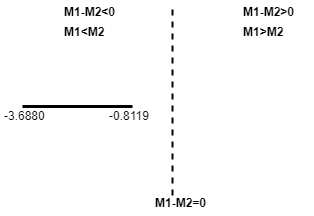
\includegraphics[width=10cm]{Figuras/Grafico3.png}
        \caption{Interpretacion intervalo para diferencia de medias en muestras relacionadas}
        \label{fig:Densidad}
    \end{center}
\end{figure}

~\\ Como asignamos una confianza del $95\%$ a nuestro intervalo, quiere decir que el $95\%$ de las veces que se repita el experimento, la diferencia real de las medias va a caer entre (-3.6880 y -0.8119). Al ver la imagen, observamos que el intervalo obtenido no contiene al cero y ademas esta debajo de el, lo que nos indica que $\mu_2>\mu_1$, y esto nos dice que el promedio de ventas despues de la campa\~{n}a publicitaria es mayor que el promedio de ventas antes de la campa\~{n}a. 

~\\ \textbf{En conclusion, podemos decir que la campa\~{n}a publicitaria es efectiva ya que aumenta el promedio de ventas.}

\pagebreak\section{Situaci\'{o}n 4}
\subsection{Punto a.}
\subsection{Punto b.}
\subsection{Punto c.}

\pagebreak\section{Situaci\'{o}n 5}



\pagebreak\section{Situaci\'{o}n 6}
\subsection{Punto a.}
~\\ Para darnos cuenta si las varianzas se puden considerar como iguales o diferentes, debemos encontrar un intervalo de confianza para la razon de las varianzas.
~\\ Extrayendo la informacion del enunciado, tenemos:
~\\ $1-\alpha=0.98$ entonces $\alpha=0.02$
~\\ Ahora, la formula para obtener un intervalo de confianza para la razon de varianzas es:

~\\ $IC(\frac{\sigma_1^{2}}{\sigma_2^{2}})_{(1-\alpha)\%}=\left[\frac{S_{1} ^{2}}{S_{2} ^{2}}\cdot F_{(\frac{\alpha}{2},n_{2}-1,n_{1}-1)}  ; \frac{S_{1} ^{2}}{S_{2} ^{2}}\cdot F_{(1-\frac{\alpha}{2},n_{2}-1,n_{1}-1)} \right]$

~\\ Hallamos $S_{1}^2$ y $S_{2}^2$:
~\\ $S_{1}^2=\frac{\sum\limits_{i=1}^{10}(x_{1i}-\bar{x_1})^2}{9}=76875.9550$ y $S_{2}^2=\frac{\sum\limits_{i=1}^{8}(x_{2i}-\bar{x_2})^2}{7}=1044021.331$
~\\ Reemplazando todo en la formula del intervalo, nos queda:

~\\ $IC(\frac{\sigma_1^{2}}{\sigma_2^{2}})_{98\%}=\left[\frac{76875.9550}{1044021.331}\cdot F_{(0.01,7,9)}  ; \frac{76875.9550}{1044021.331}\cdot F_{(0.99,7,9)} \right]$

~\\ $IC(\frac{\sigma_1^{2}}{\sigma_2^{2}})_{98\%}=[0.0765\cdot0.14884  ;  0.0765\cdot5.61287]$

~\\ $IC(\frac{\sigma_1^{2}}{\sigma_2^{2}})_{98\%}=[0.01138 ; 0.42938]$
~\\ Para interpretar mas facilmente el intervalo obtenido, hicimos la siguiente grafica:
\begin{figure}[!h]
    \begin{center}
        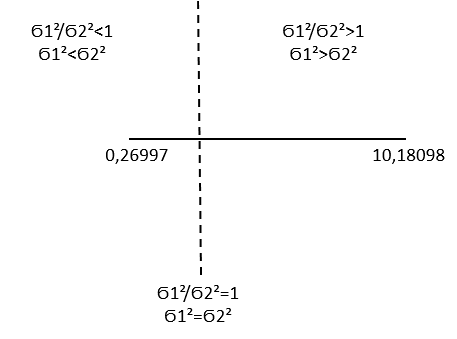
\includegraphics[width=10cm]{Figuras/Grafico4.png}
        \caption{Interpretacion intervalo para la razon de varianzas}
        \label{fig:Densidad}
    \end{center}
\end{figure}
~\\ Como asignamos una confianza del $98\%$ quiere decir, que el $98\%$ de las veces que se repita el experimento con las mismas condiciones, la razon de varianzas poblacionales va a estar entre (0.01138 y 0.42938). Si nos fijamos en la imagen, vemos que el intervalo no contiene al 1, y cae por debajo de el. Entonces concluimos que no se pueden considerar las varianzas poblacionales como iguales, y se tiene fuerte evidencia de que $\sigma_{1}^2<\sigma_{2}^2$.
\subsection{Punto b.}
~\\ Para recomendar o no el uso del revestimiento como mecanismo complementario, encontraremos un intervalo de confianza para diferencia de medias, y asi darnos cuenta si la resistencia promedio de las tuberias aumento, disminuyo, o se mantuvo igual.
~\\ Como informacion tenemos: $\bar{x_1}=2902.8$ , $\bar{x_2}=2783.125$, $S_{1}^2=76875.9550$ y $S_{2}^2=1044021.331$

~\\ Debemos aplicar la estimacion para diferencia de medias con $\sigma_{1}^2$ y $\sigma_{2}^2$ desconocidas pero diferentes, ya que en el punto anterior, mostramos que con una confianza del $98\%$ las varianzas poblacionales no van a ser iguales.
~\\ Sustituyendo los valores en la formula, tenemos:

~\\ $IC(\mu_1 - \mu_2)_{98\%}=(2902.8-2783.125)\pm t_{(0.99;16)}\cdot Sp\sqrt{\frac{1}{10}+\frac{1}{8}}$ 

~\\ Debemos hallar Sp:
~\\ $Sp=\sqrt{\frac{(n_{1}-1)S_{1}^2+(n_{2}-1)S_{2}^2}{n_{1}+n_{2}-2}}=\sqrt{\frac{9\cdot76875,9550+7\cdot1044021,331}{10+8-2}}=\sqrt{500002.057}=707.1082$

~\\ Ahora, reemplazando todo, nos queda:

~\\ $IC(\mu_1 - \mu_2)_{98\%}=[119.675 \pm 2.58349 \cdot 707.1082 \cdot 0.47434]$

~\\ $IC(\mu_1 - \mu_2)_{98\%}=[-746.8526 ; 986.2026]$

\pagebreak
~\\ \textbf{INTERPRETACION:}

~\\ Para interpretar mas facilmente el intervalo obtenido, elaboramos la siguiente grafica:
\begin{figure}[!h]
    \begin{center}
        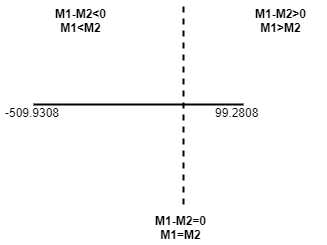
\includegraphics[width=10cm]{Figuras/Grafico5.png}
        \caption{Interpretacion intervalo para diferencia de medias en muestras independientes}
        \label{fig:Densidad}
    \end{center}
\end{figure}
~\\ Como el intervalo encontrado tiene una confianza del $98\%$, decimos que el $98\%$ de las veces que se repita el experimento en las mismas condiciones, la diferencia de medias de resistencia reales va a caer entre -746.8526 y 986.2026. Ademas, si detallamos la imagen, podemos ver que el intervalo obtenido contiene al cero, esto quiere decir que $\mu_1=\mu_2$ o son muy cercanos. Por lo que concluimos que el uso del revestimiendo no eleva la resistencia promedio de las tuberias, y no es recomendable el uso de este como mecanismo complementario.

\pagebreak\section{Situaci\'{o}n 7}
\subsection{Punto a.}
\subsection{Punto b.}
\subsection{Punto c.}

\bibliography{Bibliografia}
\end{document}